%
% CHAPTER Versuch 2
%
\chapter{Zeitverhalten der DA wandlung}
Ziel dieser Aufgabe ist es, eine Sinusspannung durch sequentiell hintereinander auf die Karte gelegte Werte zu simulieren:
\label{chap:ZeitverhaltenDA}
\section{Fragestellung, Messprinzip, Aufbau, Messmittel}
\label{chap:VERSUCH_4_FRAGESTELLUNG}
Zur bearbeitung dieser Aufgabe wird zunächst ein Pythonscript erstelt, welches Digitale Werte einer Sinusschwingung errechnet und diese anschließend mit der Funktion $rl.cbVOut(0,0,101,np.sin(x)+2)$ an den DA wandler ausgibt. Die Werte von x befinden sich gleichmäßig verteilt zwischen $-Pi$ und $+Pi$. Das Ergebnis der Sinusfunktion wird noch +2 gerechnet, damit wir in keinem Fall einen Wert kleiner Null erhalten. anschließend ist noch zu beachten, dass nach jedem aufrufen dieser Methode das Pythonmodul einen kleinen Moment schlafen sollte, damit das Signal einen Moment anliegt und anhand des Oszilloskop besser interpretiert werden kann.
\section{Ergebnis}
\label{chap:VERSUCH_4_MESSWERTE}

\begin{figure}[H]
\centering
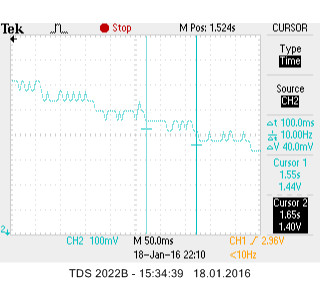
\includegraphics[width=0.75\textwidth]{sinus10Hz.jpg}
\caption{Ausgabe des Oszilloskops}
\label{fig:Oszi}
\end{figure}


\section{Auswertung und Interpretation}
\label{chap:V4_AUSWERTUNGUNDINTERPRETATION}
In Abbildung \ref{fig:Oszi} ist zu erkennen, dass unser Pythonscript nach anlegen eines neuen Pegels 100ms schläft, bevor es diesen wieder ändert.
Zwischen den beiden Linien befindet sich eine Stufe der Sinusschwingung, bei dieser ist zu erkennen, dass es sich nicht um eine  gerade handelt, sondern dass diese zwischen zwei werten schwankt. Bei dieser Schwankung handelt es sich um den zuvor errechneten Quantisierungsfehler. Dieses Verhalten ist nicht weiter verwunderlich und das schwanken von etwa 40 mV deckt sich mit dem errechneten Wert.
